\documentclass{article}
\usepackage{tikz}
\usepackage{pgfplots}
\usepackage{textcomp}
\usepackage{array}
\usepackage{tabu}
\usepackage{numprint}
\begin{document}

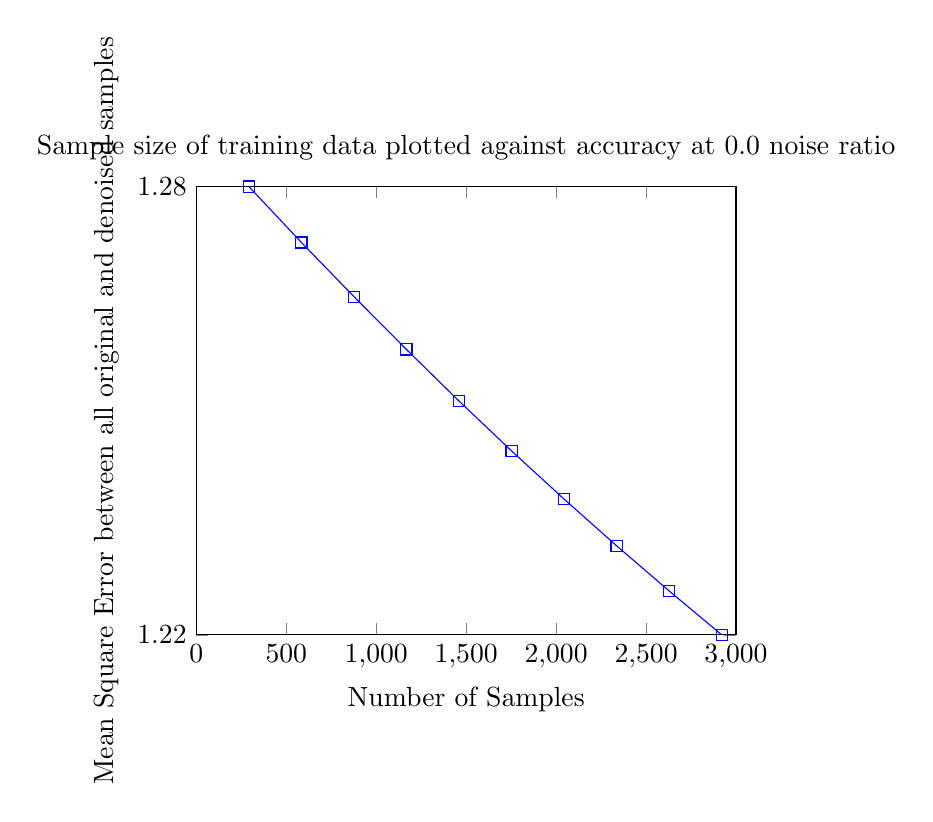
\begin{tikzpicture}
\begin{axis}[
title={Sample size of training data plotted against accuracy at 0.0 noise ratio},
xlabel={Number of Samples},
ylabel={Mean Square Error between all original and denoised samples},
xmin=0, xmax=3000,
ymin=1.2230142373707413, ymax=1.2802191646958816,
xtick={0,500,1000,1500,2000,2500,3000},
ytick={1.2230142373707413,1.2802191646958816},
legend pos=north west,
ymajorgrids=true,
grid style=dashed,
]

\addplot[
color=blue,
mark=square,
]
coordinates {

(292, 1.2802191646958816)
(584, 1.2730827458393412)
(876, 1.266172675785493)
(1168, 1.2594315363750532)
(1460, 1.2528569714406512)
(1752, 1.2464893953670837)
(2044, 1.2403444962720958)
(2336, 1.2343867447569805)
(2628, 1.228624626621504)
(2921, 1.2230142373707413)
    };
\end{axis}
\end{tikzpicture}

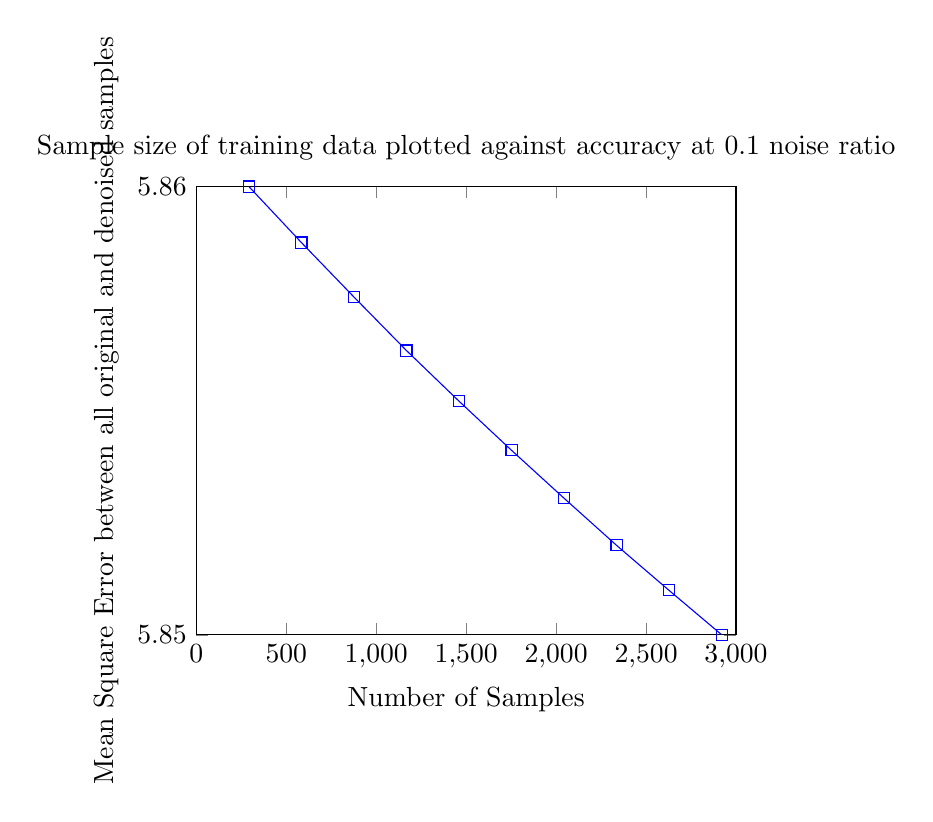
\begin{tikzpicture}
\begin{axis}[
title={Sample size of training data plotted against accuracy at 0.1 noise ratio},
xlabel={Number of Samples},
ylabel={Mean Square Error between all original and denoised samples},
xmin=0, xmax=3000,
ymin=5.854987847759298, ymax=5.864544481518619,
xtick={0,500,1000,1500,2000,2500,3000},
ytick={5.854987847759298,5.864544481518619},
legend pos=north west,
ymajorgrids=true,
grid style=dashed,
]

\addplot[
color=blue,
mark=square,
]
coordinates {

(292, 5.864544481518619)
(584, 5.863350393069998)
(876, 5.862190107966172)
(1168, 5.861048966865697)
(1460, 5.859969982952167)
(1752, 5.858922249688059)
(2044, 5.85790109854072)
(2336, 5.856895907450237)
(2628, 5.855935752588757)
(2921, 5.854987847759298)
    };
\end{axis}
\end{tikzpicture}

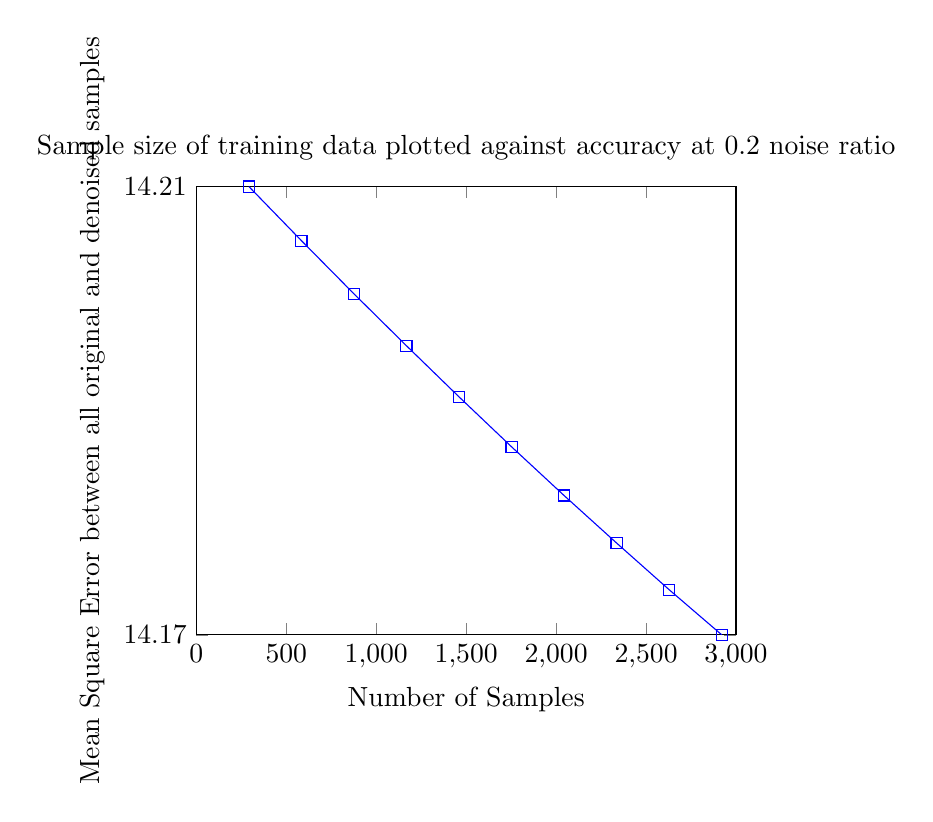
\begin{tikzpicture}
\begin{axis}[
title={Sample size of training data plotted against accuracy at 0.2 noise ratio},
xlabel={Number of Samples},
ylabel={Mean Square Error between all original and denoised samples},
xmin=0, xmax=3000,
ymin=14.168168905571664, ymax=14.208008054374634,
xtick={0,500,1000,1500,2000,2500,3000},
ytick={14.168168905571664,14.208008054374634},
legend pos=north west,
ymajorgrids=true,
grid style=dashed,
]

\addplot[
color=blue,
mark=square,
]
coordinates {

(292, 14.208008054374634)
(584, 14.203201046737927)
(876, 14.198474586431576)
(1168, 14.193860911980059)
(1460, 14.18932237620351)
(1752, 14.184885844518902)
(2044, 14.180556098326385)
(2336, 14.176333484869772)
(2628, 14.172187824554275)
(2921, 14.168168905571664)
    };
\end{axis}
\end{tikzpicture}


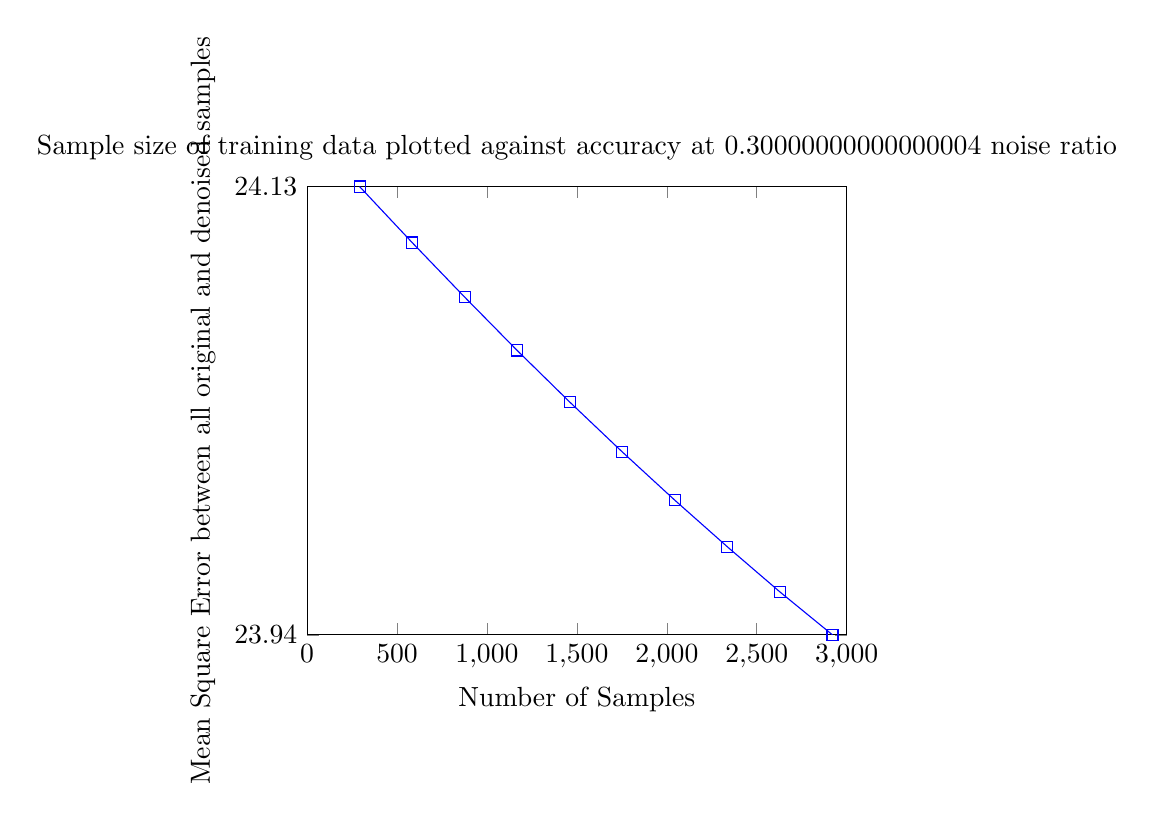
\begin{tikzpicture}
\begin{axis}[
title={Sample size of training data plotted against accuracy at 0.30000000000000004 noise ratio},
xlabel={Number of Samples},
ylabel={Mean Square Error between all original and denoised samples},
xmin=0, xmax=3000,
ymin=23.935912873669174, ymax=24.129481584515855,
xtick={0,500,1000,1500,2000,2500,3000},
ytick={23.935912873669174,24.129481584515855},
legend pos=north west,
ymajorgrids=true,
grid style=dashed,
]

\addplot[
color=blue,
mark=square,
]
coordinates {

(292, 24.129481584515855)
(584, 24.10531750953635)
(876, 24.081761721737752)
(1168, 24.05872047237489)
(1460, 24.036461733841)
(1752, 24.014925743388943)
(2044, 23.9940873098549)
(2336, 23.973980024109924)
(2628, 23.954507650082903)
(2921, 23.935912873669174)
    };
\end{axis}
\end{tikzpicture}

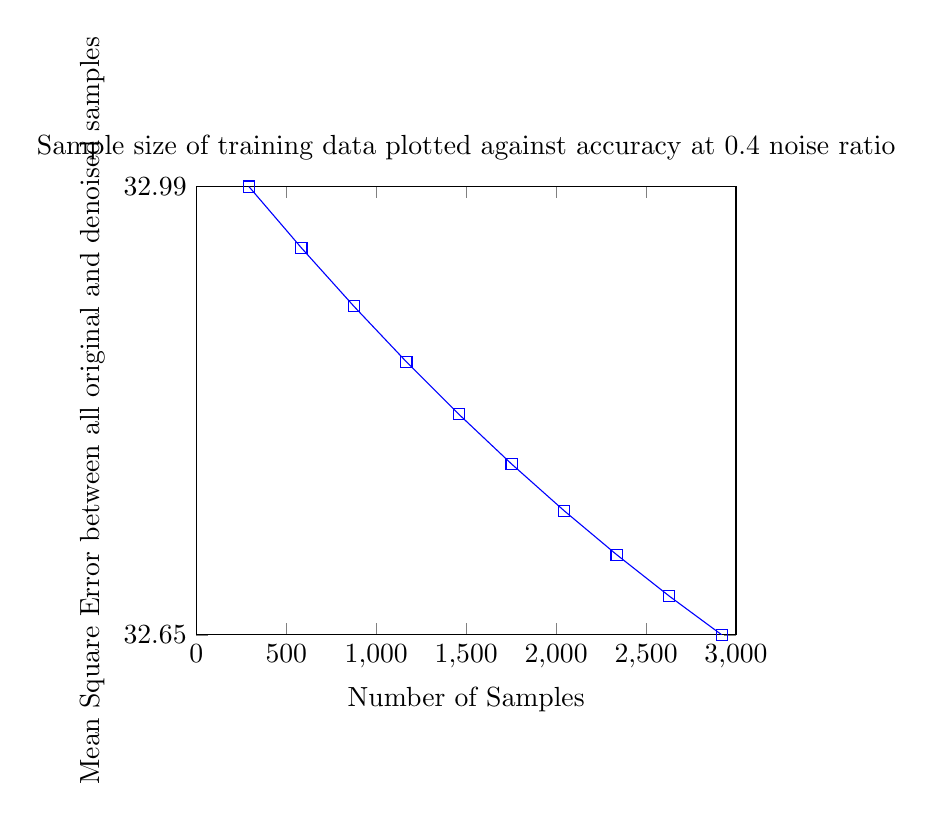
\begin{tikzpicture}
\begin{axis}[
title={Sample size of training data plotted against accuracy at 0.4 noise ratio},
xlabel={Number of Samples},
ylabel={Mean Square Error between all original and denoised samples},
xmin=0, xmax=3000,
ymin=32.647222775579536, ymax=32.98587383425296,
xtick={0,500,1000,1500,2000,2500,3000},
ytick={32.647222775579536,32.98587383425296},
legend pos=north west,
ymajorgrids=true,
grid style=dashed,
]

\addplot[
color=blue,
mark=square,
]
coordinates {

(292, 32.98587383425296)
(584, 32.93954697898185)
(876, 32.89540374165552)
(1168, 32.85343091857612)
(1460, 32.8137698352244)
(1752, 32.77634788473045)
(2044, 32.74105525869336)
(2336, 32.707858423936145)
(2628, 32.67660977273878)
(2921, 32.647222775579536)
    };
\end{axis}
\end{tikzpicture}

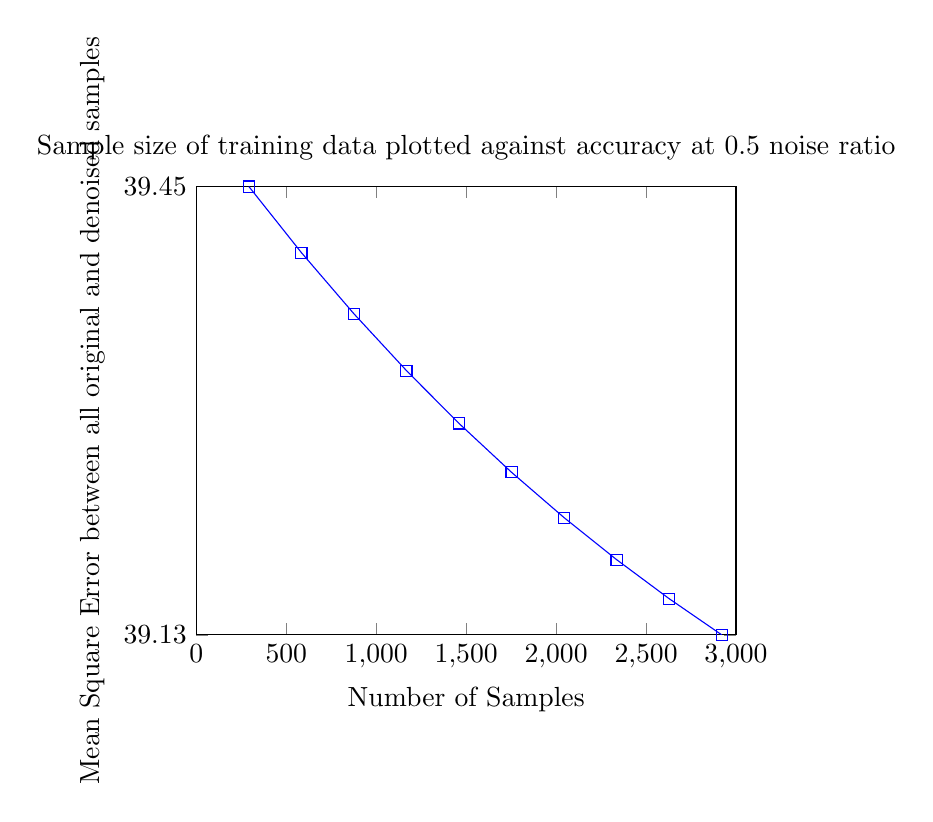
\begin{tikzpicture}
\begin{axis}[
title={Sample size of training data plotted against accuracy at 0.5 noise ratio},
xlabel={Number of Samples},
ylabel={Mean Square Error between all original and denoised samples},
xmin=0, xmax=3000,
ymin=39.132875107114785, ymax=39.453181083316956,
xtick={0,500,1000,1500,2000,2500,3000},
ytick={39.132875107114785,39.453181083316956},
legend pos=north west,
ymajorgrids=true,
grid style=dashed,
]

\addplot[
color=blue,
mark=square,
]
coordinates {

(292, 39.453181083316956)
(584, 39.405969388248614)
(876, 39.36226752641123)
(1168, 39.321684014764585)
(1460, 39.283960105602915)
(1752, 39.24904534780458)
(2044, 39.21667012875412)
(2336, 39.186649994480526)
(2628, 39.15877017662976)
(2921, 39.132875107114785)
    };
\end{axis}
\end{tikzpicture}


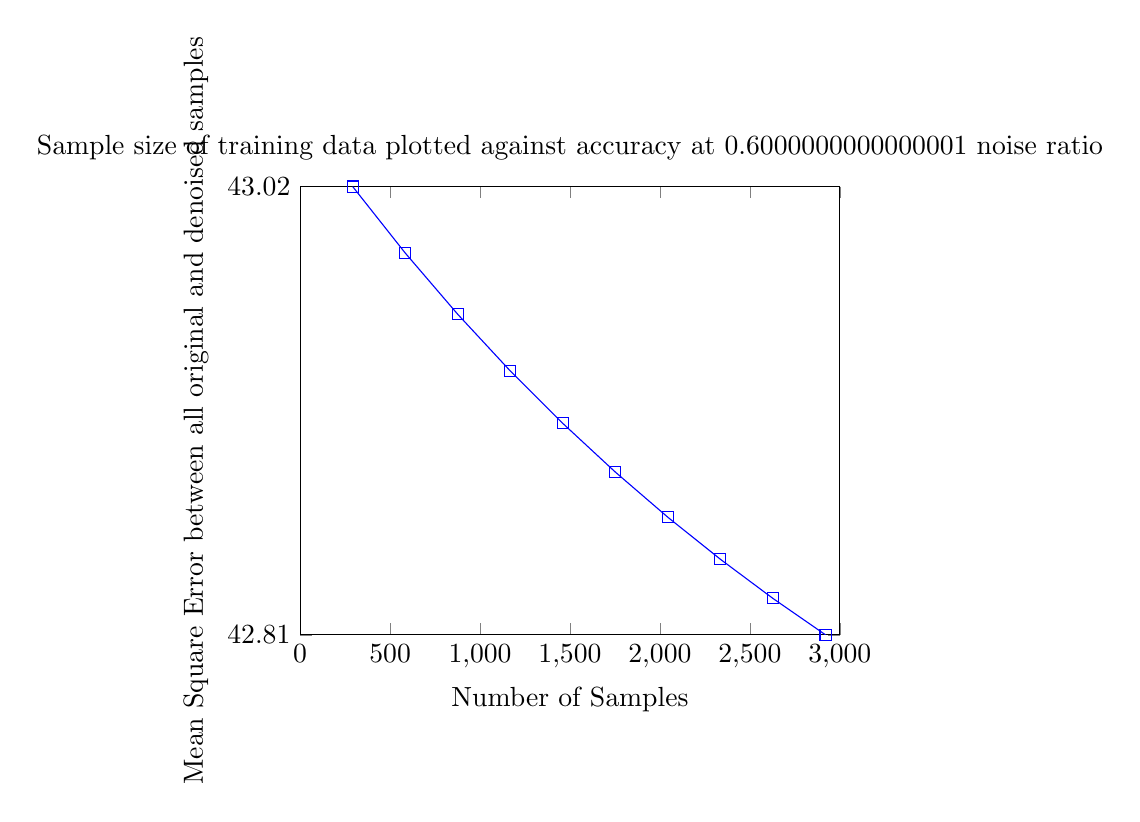
\begin{tikzpicture}
\begin{axis}[
title={Sample size of training data plotted against accuracy at 0.6000000000000001 noise ratio},
xlabel={Number of Samples},
ylabel={Mean Square Error between all original and denoised samples},
xmin=0, xmax=3000,
ymin=42.811015075820926, ymax=43.01730013660565,
xtick={0,500,1000,1500,2000,2500,3000},
ytick={42.811015075820926,43.01730013660565},
legend pos=north west,
ymajorgrids=true,
grid style=dashed,
]

\addplot[
color=blue,
mark=square,
]
coordinates {

(292, 43.01730013660565)
(584, 42.98673950815356)
(876, 42.958535536169066)
(1168, 42.93247054593745)
(1460, 42.90834309985616)
(1752, 42.885944971247284)
(2044, 42.86515097140032)
(2336, 42.845828409919314)
(2628, 42.82781001159111)
(2921, 42.811015075820926)
    };
\end{axis}
\end{tikzpicture}


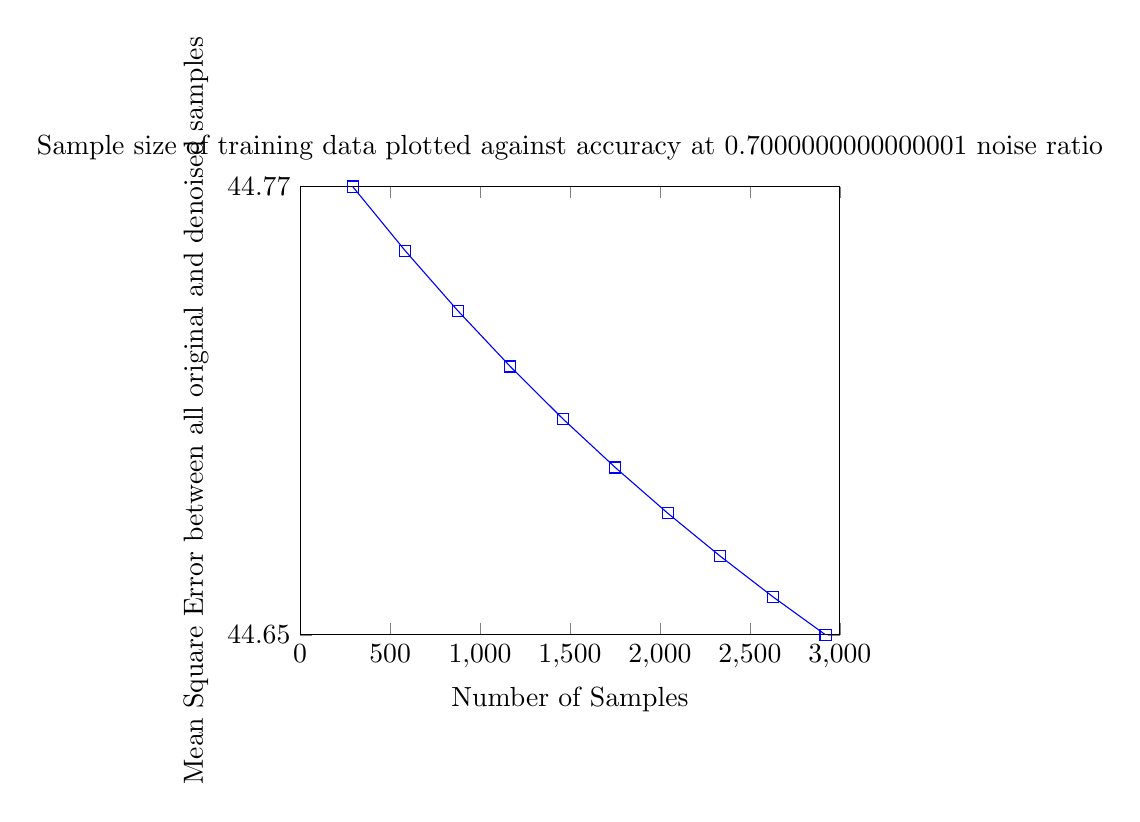
\begin{tikzpicture}
\begin{axis}[
title={Sample size of training data plotted against accuracy at 0.7000000000000001 noise ratio},
xlabel={Number of Samples},
ylabel={Mean Square Error between all original and denoised samples},
xmin=0, xmax=3000,
ymin=44.650881066594486, ymax=44.774317879948015,
xtick={0,500,1000,1500,2000,2500,3000},
ytick={44.650881066594486,44.7743178799480157},
legend pos=north west,
ymajorgrids=true,
grid style=dashed,
]

\addplot[
color=blue,
mark=square,
]
coordinates {

(292, 44.774317879948015)
(584, 44.756646603579306)
(876, 44.740158982477006)
(1168, 44.72477898834629)
(1460, 44.7103938903745)
(1752, 44.696966379481566)
(2044, 44.68436333650364)
(2336, 44.672528857892246)
(2628, 44.66137591778634)
(2921, 44.650881066594486)
    };
\end{axis}
\end{tikzpicture}


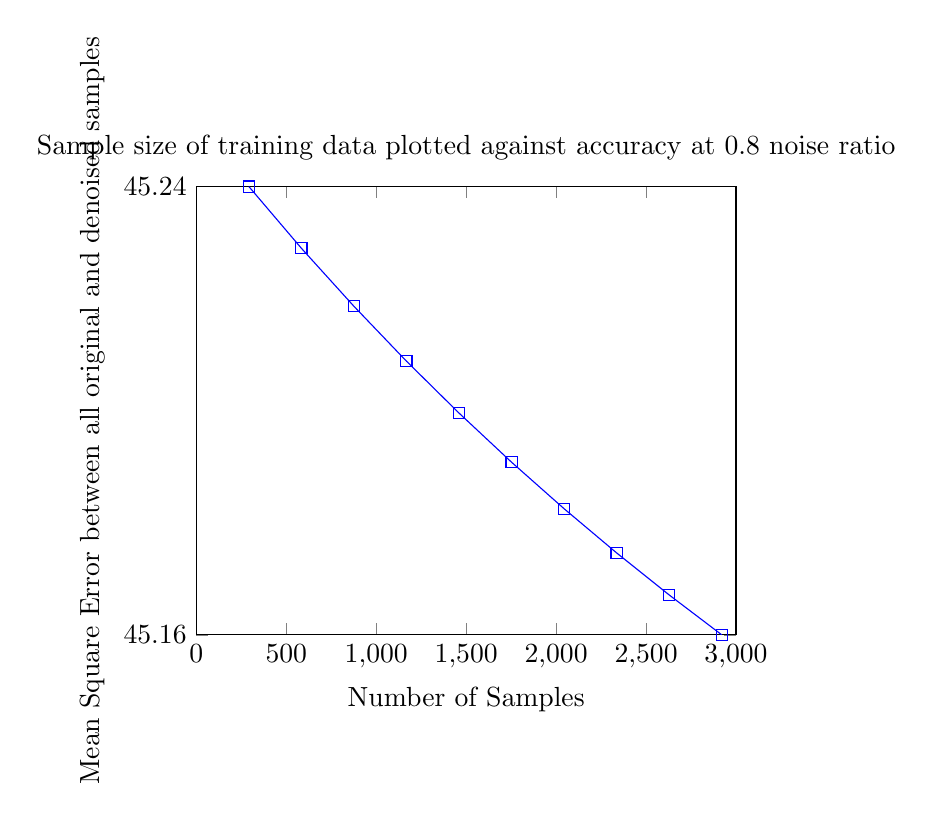
\begin{tikzpicture}
\begin{axis}[
title={Sample size of training data plotted against accuracy at 0.8 noise ratio},
xlabel={Number of Samples},
ylabel={Mean Square Error between all original and denoised samples},
xmin=0, xmax=3000,
ymin=45.164558538153464, ymax=45.23767992479124,
xtick={0,500,1000,1500,2000,2500,3000},
ytick={45.164558538153464,45.23767992479124},
legend pos=north west,
ymajorgrids=true,
grid style=dashed,
]

\addplot[
color=blue,
mark=square,
]
coordinates {

(292, 45.23767992479124)
(584, 45.22761112722728)
(876, 45.21815164447122)
(1168, 45.20919822271562)
(1460, 45.20074009003918)
(1752, 45.19272825569556)
(2044, 45.18514196006417)
(2336, 45.17793481829655)
(2628, 45.171082213493804)
(2921, 45.164558538153464)
    };
\end{axis}
\end{tikzpicture}

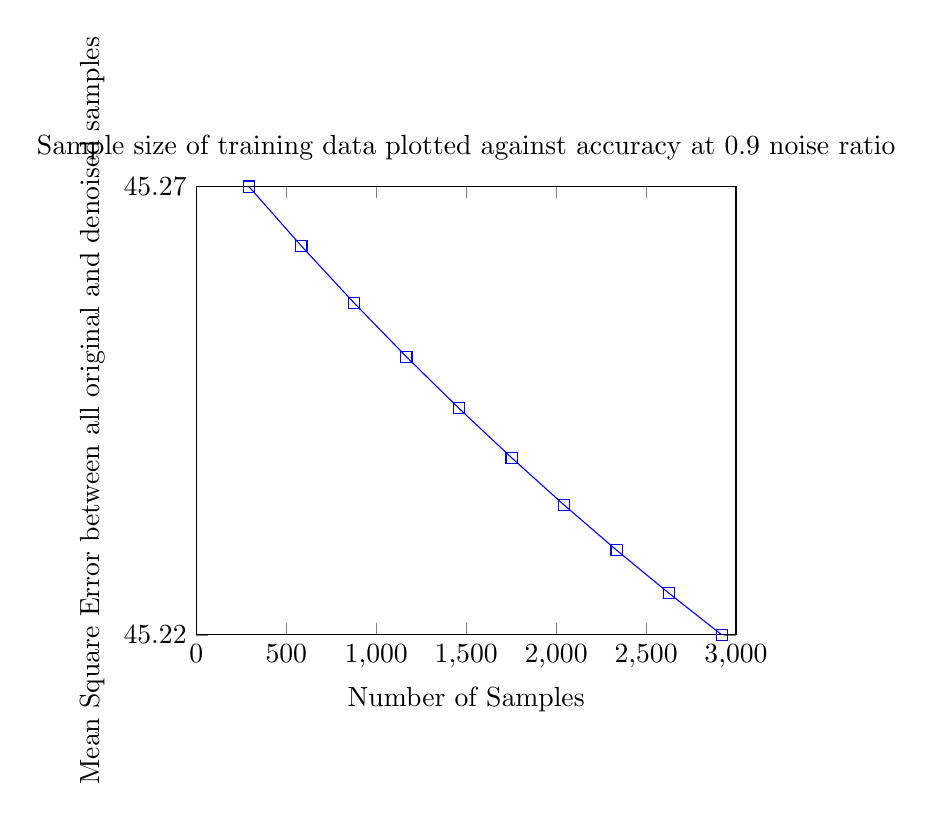
\begin{tikzpicture}
\begin{axis}[
title={Sample size of training data plotted against accuracy at 0.9 noise ratio},
xlabel={Number of Samples},
ylabel={Mean Square Error between all original and denoised samples},
xmin=0, xmax=3000,
ymin=45.2222520919187, ymax=45.26908812596585,
xtick={0,500,1000,1500,2000,2500,3000},
ytick={45.2222520919187,45.26908812596585},
legend pos=north west,
ymajorgrids=true,
grid style=dashed,
]

\addplot[
color=blue,
mark=square,
]
coordinates {

(292, 45.26908812596585)
(584, 45.26287164569183)
(876, 45.256946400354096)
(1168, 45.2512991610618)
(1460, 45.24591816385284)
(1752, 45.24076420270186)
(2044, 45.235823783904245)
(2336, 45.23110495455972)
(2628, 45.22659171356147)
(2921, 45.2222520919187)
    };
\end{axis}
\end{tikzpicture}

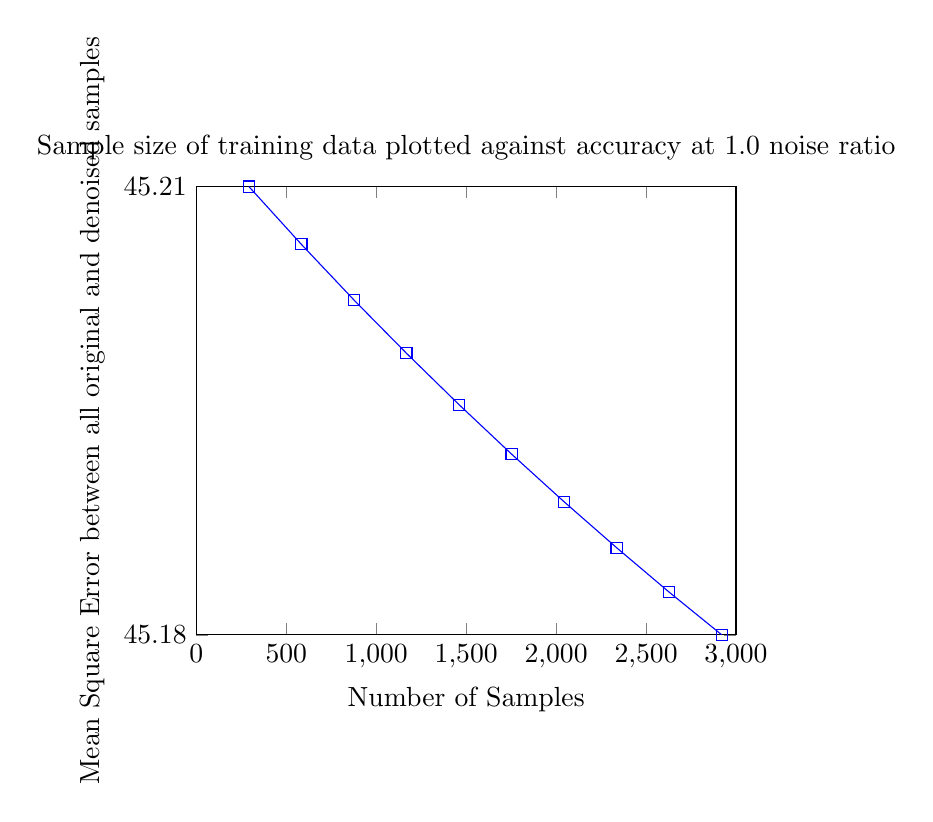
\begin{tikzpicture}
\begin{axis}[
title={Sample size of training data plotted against accuracy at 1.0 noise ratio},
xlabel={Number of Samples},
ylabel={Mean Square Error between all original and denoised samples},
xmin=0, xmax=3000,
ymin=45.18042660213684, ymax=45.21171264190544,
xtick={0,500,1000,1500,2000,2500,3000},
ytick={45.18042660213684,45.21171264190544,45.242998681674045},
legend pos=north west,
ymajorgrids=true,
grid style=dashed,
]

\addplot[
color=blue,
mark=square,
]
coordinates {

(292, 45.21171264190544)
(584, 45.2076764839328)
(876, 45.20379775343453)
(1168, 45.2000786693421)
(1460, 45.196496449275536)
(1752, 45.193045203031936)
(2044, 45.18971780985)
(2336, 45.186512991234935)
(2628, 45.18341269255011)
(2921, 45.18042660213684)
    };
\end{axis}
\end{tikzpicture}

\end{document}